\subsection{Generator Constant} %\label{put a label here and uncomment}
\textbf{Name: Group 510}\\
\textbf{Date: 30/09 - 2015}

\subsubsection{Purpose}
The purpose of the test is to find the generator constant $K_e$ by measuring the motor voltages, currents and velocities, in several steady states.

\subsubsection{Setup}
\begin{figure}[H]
  \centering
	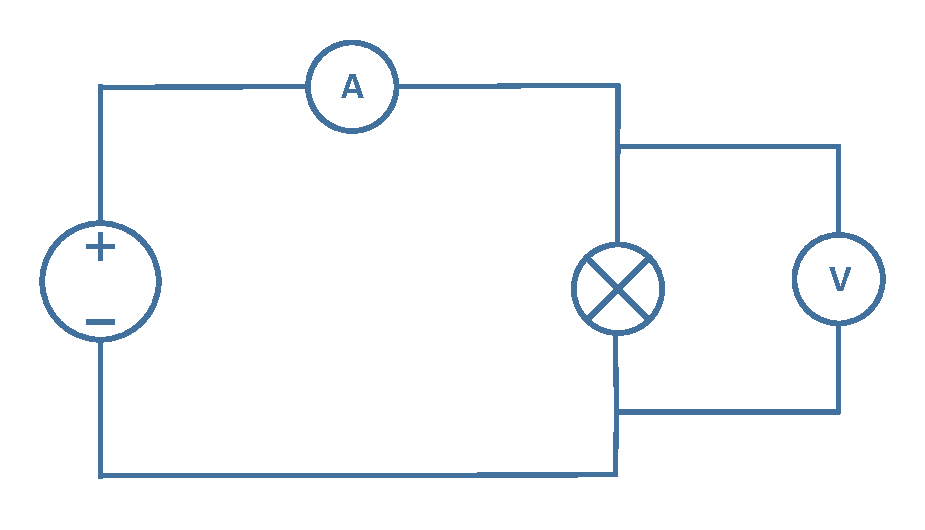
\includegraphics[scale=0.5]{figures/MotorTest4.pdf}
	\caption{Use-Case Diagram}
\end{figure}

\subsubsection{List of Equipment}

\begin{table}[H]
\begin{tabular}{|l|l|p{4cm}|}
\hline%------------------------------------------------------------------------------------
  \textbf{Instrument}                        &  \textbf{AAU-no.}  &  \textbf{Type}       \\
\hline%------------------------------------------------------------------------------------
  Multimeter 1                               &  60764             &  Fluke 189 True RMS  \\
\hline%------------------------------------------------------------------------------------
  Multimeter 2                   		         &  60769             &  Fluke 189 True RMS  \\
\hline%------------------------------------------------------------------------------------
  Power Supply ($0 - 32$ V) ($0 - 10$ A)     &  77076             &  Ea - ps 7032 - 100  \\
\hline%------------------------------------------------------------------------------------
  Optical tachometer                         &  08246             &  Shimpo DT-205       \\
\hline%------------------------------------------------------------------------------------
\end{tabular}
\end{table}

\subsubsection{Procedure}

\begin{enumerate}
  \item Turn on the two multimeters and put them in ampere and voltage mode respectively.
  \item Apply $1$ V by use of the voltage mode multimeter
  \item Read out the current value from the ampere mode multimeter
  \item Read out RPM of the motor using the optical tachometer.
  \item Repeat the past $3$ steps up to $7$ V in $1$ V increments.
\end{enumerate}

\subsubsection{Results}

\begin{table}[H]
\begin{tabular}{|l|l|l|}
\hline%----------------------------------------------------------------
  \textbf{Input (V)}  & \textbf{Output (A)} & \textbf{Output (RPM)} \\
\hline%----------------------------------------------------------------
  $1$                 &            $1.7$  &  $3684$                 \\
\hline%----------------------------------------------------------------
  $2$                 &            $2.2$  &  $8063$                 \\
\hline%----------------------------------------------------------------
  $3$                 &            $2.6$  &  $12021$                \\
\hline%----------------------------------------------------------------
  $4$                 &            $3.3$  &  $16746$                \\
\hline%----------------------------------------------------------------
  $5$                 &            $4.1$  &  $21966$                \\
\hline%----------------------------------------------------------------
  $6$                 &            $4.8$  &  $26420$                \\
\hline%----------------------------------------------------------------
  $7$                 &            $5.6$  &  $31447$                \\
\hline%----------------------------------------------------------------
\end{tabular}
\end{table}

$K_e = \frac{U_a - R_a I_a}{\omega}$.